\documentclass[a4paper]{article}

\usepackage{pdflscape}
\usepackage{multicol}
\usepackage{blindtext}
\usepackage{color}
\usepackage{enumitem}

\usepackage[left=10mm, right=10mm, top=10mm, bottom=10mm]{geometry}

\usepackage{titlesec}

\usepackage[utf8]{inputenc}
\usepackage{fourier} 
\usepackage{array}
\usepackage{makecell}

\usepackage[demo]{graphicx}



\renewcommand\theadalign{bc}
\renewcommand\theadfont{\bfseries}
\renewcommand\theadgape{\Gape[4pt]}
\renewcommand\cellgape{\Gape[4pt]}

\titlespacing\section{0pt}{5pt plus 4pt minus 2pt}{0pt plus 2pt minus 2pt}
\titlespacing\subsection{0pt}{5pt plus 4pt minus 2pt}{0pt plus 2pt minus 2pt}
\titlespacing\subsubsection{0pt}{5pt plus 4pt minus 2pt}{0pt plus 2pt minus 2pt}

\newenvironment{Figure}
  {\par\medskip\noindent\minipage{\linewidth}}
  {\endminipage\par\medskip}


\setlength{\columnseprule}{0.5pt}
\def\columnseprulecolor{\color{black}}

\pagenumbering{gobble}

\title{MuDa Cheat Sheet}
\author{Niklas Ullmann}
\date{Summer 2022}

%

\begin{document}
\begin{landscape}
    \thispagestyle{empty}

    \begin{multicols}{3}
        %
        %   Grundlagen
        %
        \section{Grundlagen}
        \begin{itemize}[noitemsep,nolistsep,leftmargin=*]
            \item Grundlagen
            \begin{itemize}[noitemsep,nolistsep,leftmargin=*]
                \item\textbf{ $Y = f(x) + \epsilon$}
                \item $Y$ = Zielgröße, $f()$ = unbekanntes/wahres Modell, $X$ = Prädiktoren, $\epsilon$ Nicht reduzierbarer Fehler
                \item \textbf{$\hat{Y} = \hat{f}(X)+\epsilon$}
                \item $\hat{Y}$ = Schätzung der Zielgröße, $\hat{f}$ = Schätzung des Modells
                \item Ziel: Möglichst genaue Schätzung finden
            \end{itemize}
            \item Ziel:
            \begin{itemize}[noitemsep,nolistsep,leftmargin=*]
                \item Prediction (Vorhersage von Werten)
                \item Inference (Ursachenanalyse, wie wirken sich Änderungen aus)
            \end{itemize}
            \item Bias-Variance Tradeoff
            \begin{itemize}[noitemsep,nolistsep,leftmargin=*]
                \item Bias: Fähigkeit des Models die eigentliche Beziehung der Daten abzubilden
                \item Variance: Fähigkeit des Models auf anderen Subsets gleich gute Modelle zu erzeugen
                \item TrainingsError: Wird immer kleiner, da Modell sich immer besser anpasst
                \item TestError: Wird erst kleiner, steigt dann aber wieder (Overfitting)
                \item Nichtreduzierbarer Error: Bleibt immer gleich (Messfehler etc.)
            \end{itemize}
        \end{itemize}
        \begin{Figure}
            \centering
            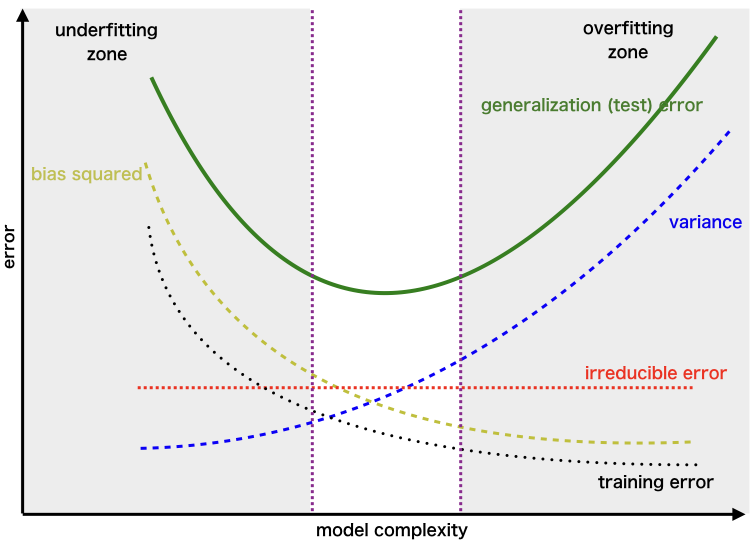
\includegraphics[width=0.75\linewidth]{bv_tradeoff.png}
        \end{Figure}



        %
        %   Regression
        %
        \section{Regression}
        \begin{itemize}[noitemsep,nolistsep,leftmargin=*]
            \item Modellgüte:
            \begin{itemize}[noitemsep,nolistsep,leftmargin=*]
                \item Schätzung der Parameter $\beta_0 und \beta_1$ über kleinste Quadrate
                \begin{itemize}[noitemsep,nolistsep,leftmargin=*]
                    \item $\beta_1 = \frac{\sum_{i=1}^{n}(x_i-\overline{x})*(y_i-\overline{y})}{\sum_{i=1}^{n}(x_1-\overline{x})^2}$ 
                    \item $\beta_0 = \overline{y} - \beta_1\overline{x}$
                    \item Erwartungstreue: $E(\hat{\beta}_0) = \beta_0$ und $E(\hat{\beta}_1) = \beta_1$
                \end{itemize}
                \item $RSS = \sum_{i=1}^{n}(y_i-\hat{y}_i)^2$
                \item $RSE = \sqrt{\frac{1}{n-2}\sum_{i=1}^{n}(y_i-\hat{y}_i)^2}$ (Zielgröße weicht im Durchschnitt RSE Einheiten von der Regressionsgeraden ab)
                \item $R^2 = 1 - \frac{RSS}{TSS}$, je größer desto besser $0 \leq R^2 \leq 1$ (Var(Zielwert) wird durch $R^2\%$ der Prädiktoren erklärt)
                \item $R^2_{adj} = 1- \frac{(1-R^2)(N-1)}{N-p-1}$ Adjustiert mit Anzahl der Prädiktoren
                \item Standardfehler und Intervalle
                \begin{itemize}[noitemsep,nolistsep,leftmargin=*]
                    \item $Var(\epsilon)=\frac{1}{n-2}\sum_{i=1}^{n}(y_i-\hat{y}_i)^2$
                    \item $(SE(\hat{\beta}_0))^2 = Var(\epsilon)*(\frac{1}{n}+\frac{\overline{x}^2}{\sum_{i=1}^{n}(x_i-\overline{x})^2})$
                    \item $(SE(\hat{\beta}_1))^2 = \frac{Var(\epsilon)}{\sum_{i=1}^{n}(x_i-\overline{x})^2}$
                    \item Intervallschätzung: $[\hat{\beta}_1-2*SE(\hat{\beta}_1), \hat{\beta}_1+2*SE(\hat{\beta}_1)]$
                    \item Interpret: Aus 100 Proben liegt $ \beta_1$ in 95 Fällen im Interval
                    \item 95\%-Konfidenzinterval: bezieht sich auf den durchschnittlichen Y Wert
                    \item 95\%-Prognoseinterval: bezieht sich auf den konkreten Wert Y von Ausgangswerten X1\dots
                \end{itemize}
                \item t-Test
                \begin{itemize}[noitemsep,nolistsep,leftmargin=*]
                    \item $H_0: \beta_0 = 0; H_1: \beta_1 \neq 0$
                    \item $X_1$ Hat keinen Einfluss auf Y
                    \item $t = \frac{\hat{\beta_1}}{SE(\hat{\beta_1})}$
                    \item Einfach den p-Wert ablesen, wenn < als bspw. 0.05 dann $H_0$ verwerfen
                \end{itemize}
                \item F-Test
                \begin{itemize}[noitemsep,nolistsep,leftmargin=*]
                    \item $H_0: \beta_0 = \beta_1 = ... = 0$
                    \item Alle Prädiktoren haben keinen Einfluss auf Y
                \end{itemize}
            \end{itemize}
            \item Qualitative Prädiktoren:
            \begin{itemize}[noitemsep,nolistsep,leftmargin=*]
                \item \textbf{Prädiktoren mit 2 Ausprägungen:}
                \item DummyVariable aka 0(No) oder 1 (Yes)
                \item \textcolor{red}{Achte auf Normalausprägung von R}
                \item $\hat{y} = \beta_0 + \beta_1*x_i $
                \item Koeffizient $\beta_1$ kürzt sich je nach Ausprägung raus
                \item \textbf{Prädiktoren mit $k$ Ausprägungen:}
                \item Erstelle $k-1$ Dummyvariablen
                \item Andere ist Normalzustand
            \end{itemize}
            \item Interaktionseffekte:
            \begin{itemize}[noitemsep,nolistsep,leftmargin=*]
                \item Synergieeffekte zwischen zwei oder mehreren Variablen
                \item $\hat{y}=\beta_0+\beta_1x_1+\beta_2x_2+\beta_3x_1x_2+\epsilon$
                \item Auswirkung erkennen durch Umformung:
                \item $\hat{y}=\beta_0++\beta_2x_2+ (\beta_1+\beta_3x_2)*x_1$
                \item Erhöht man $x_1$ um eine Einheit erhöht sich $\hat{y}$ um $\beta_1+\beta_3x_2$ Einheiten
                \item $x_1$ moderiert $x_2$ und Vice versa
                \item Signifikanz über p-value feststellen
                \item Interaktion zwischen Qauli udn Quanti Variablen:
                \item Kürzt sich komplett raus (wenn 0) oder ist $*1$ (wenn 1)
            \end{itemize}
        \end{itemize}


        %
        %   Klassifikation
        %
        \section{Klassifikation}
        \begin{itemize}[noitemsep,nolistsep,leftmargin=*]
            \item \textbf{Grundlagen:}
            \begin{itemize}[noitemsep,nolistsep,leftmargin=*]
                \item Klassifikation ist Zuordnung von bedingten Wahrscheinlichkeiten anhand von Ausprägungen
                \item $P(Y = k | X=x)$
                \item Klasse mit höchster Wahrscheinlichkeit wird gewählt
                \item Bpsw: Y = 1 (Yes) und 0 (No)
                \begin{itemize}[noitemsep,nolistsep,leftmargin=*]
                    \item Lineare Regression, die die Wahrscheinlichkeitausgibt \textcolor{red}{funktioniert nicht!}
                    \item Reg.Gerade wird unter 0 fitten und auch nicht bis 1
                \end{itemize}
                \item Funktion finden, die $0 \leq p(x) \leq 1$ für alle X
            \end{itemize}
            \item \textbf{Logistic Regression:}
            \begin{itemize}[noitemsep,nolistsep,leftmargin=*]
                \item $p(x) = \frac{e^{\beta_0+\beta_1*X}}{1+e^{\beta_0+\beta_1*X}}$
                \item $0 \leq p(x) \leq 1$, da immer $e^x \geq 0$ und $\frac{X}{1+X}\leq 1$
                \item Odds:
                \begin{itemize}[noitemsep,nolistsep,leftmargin=*]
                    \item $\frac{p(x)}{1-(px)}= e^{\beta_0+\beta_1*X}$
                    \item $0 \leq odds \leq \infty$
                    \item Möglichkeit Wahrscheinlichkeit anzugeben:
                    \item Odds= $\frac{4}{3}$ -> "Siegchancen stehen 4 zu 3"
                    \item Umrechnung:
                    \item $p = \frac{odds}{1+odds} = \frac{e^{logit}}{1+e^{logit}}$
                    \item $odds = \frac{p}{1-p} = e^{logit}$
                \end{itemize}
                \item Logits:
                \begin{itemize}[noitemsep,nolistsep,leftmargin=*]
                    \item $log(\frac{p(x)}{1-(px)})= \beta_0+\beta_1*X$
                    \item $-\infty \leq logits \leq \infty$
                    \item Logits hängen Linear von X ab
                \end{itemize}
            \end{itemize}
            \item \textbf{Schätzung der Koeffizienten}
            \begin{itemize}[noitemsep,nolistsep,leftmargin=*]
                \item Schätzung von $\beta_0$ und $\beta_1$ über Maximum-Likelihood
                \item $l(\beta_0, \beta_1)= \Pi_{i:y_i=1} p(x_i) * \Pi_{i:y_i=0} (1-p(x_i)) $
                \item Funktion wird maximiert = da wo Likelihood am größten ist, sind Parameter am besten
            \end{itemize}
            \item \textbf{Validierung:}
            \begin{itemize}[noitemsep,nolistsep,leftmargin=*]
                \item Gleiche Werte/ Tests, wie bei lineare Regression
            \end{itemize}
            \item \textbf{Confounding:}
            \begin{itemize}[noitemsep,nolistsep,leftmargin=*]
                \item Zusammenhang zwischen zwei Prädiktoren
                \item Confounder beeinflusst gleichzeitig Zielgröße und anderen Prädiktor
                \item \textcolor{red}{Hier fehlts}
            \end{itemize}
        \end{itemize}


        %
        %   Resampling
        %
        \section{Resampling}
        \begin{itemize}[noitemsep,nolistsep,leftmargin=*]
            \item \textbf{Grundlagen:}
            \begin{itemize}[noitemsep,nolistsep,leftmargin=*]
                \item TestError wird mit ungesehenen Daten berechnet.
                \item Meist aber keine vorhanden -> TestError muss über Trainingsdaten geschätzt werden
                \item Verfahren für Regression/Klassifikation anwendbar
            \end{itemize}
            \item \textbf{Einfache Valididerung:}
            \begin{itemize}[noitemsep,nolistsep,leftmargin=*]
                \item Teile Trainingsdaten in zwei gleiche große Mengen auf
                \item Menge1: für Training / Menge2: für Testing
                \item MSE variiert stark in Abhängikeit der Traininsgmenge
                \item Modelle sollten möglichst mit hoher Trainingsmenge trainiert werden
                \item Hoher Bias, geringe Varianz
            \end{itemize}
            \item \textbf{LeaveOneOut Validierung:}
            \begin{itemize}[noitemsep,nolistsep,leftmargin=*]
                \item n-Modelle werden mit n-1 Datensätze trainiert
                \item Letzter Datensatz ist Testdatensatz
                \item Durchschnitt aller MSEs ist finaler Wert
                \item $CV_{(n)} = \frac{1}{n}\sum_{i=1}^n MSE_i$
                \item Vorteil: Größere Trainingsmenge
                \item Nachteil: Hoher Rechenaufwand für n Modelle, größere Varianz als bei einfacher Val, durch Autokorrelation
                \item geringer Bias, hohe Varianz
            \end{itemize}
            \item \textbf{k-fold Validierung}
            \begin{itemize}[noitemsep,nolistsep,leftmargin=*]
                \item Teile Datensatz in k gleich große Mengen (5, 10..)
                \item Trainiere k Modelle, wobei immer eine Teilmenge als Test genutzt wird
                \item $CV_{(k)} = \frac{1}{k}\sum_{i=1}^k MSE_i$
                \item geringere Streuung des MSEs
                \item Guter Kompromiss zwischen Rechenaufwand und guter Abschätzung
            \end{itemize}
            \item Für Klassifikation wird der Anteil falsch klassifizierter Objekte genommen!
        \end{itemize}



        %
        %   Modellauswahl
        %
        \section{Modellauswahl}
        \begin{itemize}[noitemsep,nolistsep,leftmargin=*]
            \item p (\# Prädiktoren), n (\# Beobachtungen)
            \item Steigende Varianz und sinkender Prognosegüte, wenn p -> n
            \item Hohe Anzahl an Prädiktoren: Steigende Wahrscheinlichkeit von Multikollinearitär (Abhängige Prädiktoren) und unnötige Komplexität
            \item Wenn $p \geq n $, ist Methode der kleinsten Quadrate gar nicht möglich
            \item \textbf{Best Subset Selection:}
            \begin{itemize}[noitemsep,nolistsep,leftmargin=*]
                \item Berechne alle Modelle mit k Parametern (Speicher das beste (Min. RSS oder Max. $R^2$))
                \item Berechne für k = 0,1,2 .. x alle besten Modelle
                \item Wähle beste aus Besten aus (siehe unten)
                \item Hoher Rechenaufwand ($2^p$ Modelle), Gefahr von Overfitting, findet optimales Modell
            \end{itemize} 
            \item \textbf{Forward Stepwise Selection:}
            \begin{itemize}[noitemsep,nolistsep,leftmargin=*]
                \item Berechne bestes Modell mit 0 Prädiktoren, dann mit 1, etc.
                \item Wähle für k immer das beste Modell und gehe von dort aus weiter
                \item Wähle beste aus Besten aus
                \item Weniger Rechenaufwand ($p^2$ Modelle), Overfitting unwahrscheinlich, findet nur lokales Optimum
            \end{itemize}
            \item \textbf{Backward Stepwise Selection:}
            \begin{itemize}[noitemsep,nolistsep,leftmargin=*]
                \item Wie Forward Stepwise Selection nur rückwärts
                \item Starte mit Modell mit k Prädiktoren und nimm immer den schlechtesten Weg
                \item Wähle beste aus Besten aus
                \item Weniger Rechenaufwand ($p^2$ Modelle), Overfitting unwahrscheinlich, findet nur lokales Optimum
            \end{itemize}
            \item \textbf{Bestes Modell?}
            \begin{itemize}[noitemsep,nolistsep,leftmargin=*]
                \item $R^2$ und $RSS$ ist nicht aussagekräftig, da es mit steigender Anzahl an Prädiktoren besser wird. 
                \item Testfehler indirekt messbar durch ($C_p, AIC, BIC und R^2_{adj}$) oder direkt durch Kreuzvalidierung
                \item Anwendbar bei linearen Modellen
                \item $RSS = \sum_{i=1}^{n}(y_i-\hat{y}_i)^2$
                \item n: Anzahl der Beobachtungen, d: Anzahl der Prädiktoren
                \item $\sigma^2 = Var(\epsilon) = \frac{1}{n-p-1}*RSS$  
                \item Mallows $C_p = \frac{1}{n}(RSS + 2d\sigma^2)$
                \item $AIC = \frac{1}{n\sigma^2}(RSS + 2d\sigma^2)$ (Proportional zu $C_p$)
                \item $BIC = \frac{1}{n\sigma^2}(RSS + ln(n)d\sigma^2)$ (Höheres Gewicht auf Strafterm für viel Prädiktoren)
                \item $R^2_a = R^2 - \frac{p}{n-p-1}(1-R^2)$ kann bei Hinzunahme einer Variable auch kleiner und oder negativ werden
            \end{itemize}
        \end{itemize}



        %
        %   R-Hilfe
        %
        \section{R - Hilfe}
        \begin{itemize} [noitemsep,nolistsep,leftmargin=*]
            \item \textbf{Grundlagen:}
            \begin{itemize}[noitemsep,nolistsep,leftmargin=*]
                \item $set.seed(X)$ Setzt Seed für random Number Generator
                \item $c(1,2,3,4)$ Vektor mit Zahlen 1-4
                \item $rep(1:10, 100)$ Erzeugt Vektor mit zahlen 1-10, 100 mal
                \item $rnorm(100)$ Erzeugt Vektor mit 100 normalverteilten Werten
                \item $runif(X, a,b)$Erzeugt X Zufallszahlen zwischen a und b
                \item $df[2,3]$ Greift auf Element der 2.Reihe und 3.Spalte des DFs zu
                \item $df[,-3]$ Entfernt 3. Spalte
                \item $head()$ Zeigt erste X Zeilen von DF an
                \item $summary()$ gibt Zusammenfassung von Modellen (DF, Modelle etc.)
                \item $table(X,Y)$ gibt Tabelle bzw. Konfusionsmatrix aus
                \item $nrow(X)$ gibt Anzahl der Zeilen in X
                \item $sample(n, n/2)$ gibt 50\% Subsetvektor
                \item $is.na(X)$ findet/zählt null Values
                \item $na.omit(X)$ entfernt null Values
                \item $var(X), mean(X)$ Varianz und Durchschnitt von X
            \end{itemize}

            \item \textbf{Modelle:}
            \begin{itemize}[noitemsep,nolistsep,leftmargin=*]
            \item $lm(A ~ B + poly(C,2) + BC, data = \dots, subset=)$ Lineare Regression für A mit Interaktivität von BC und C mit Exponent 2
            \item $glm(A ~ B + C, data=\dots, family = binomial, subset=)$ Logistic Regression Modell
            \item $predict(Modell, DataFrame, interval= , type= )$
                \begin{itemize}[noitemsep,nolistsep,leftmargin=*]
                    \item DF: $data.frame(x1 = c(2), x2 = c(3))$ 
                    \item $interval$ Konfidenzinterval(confidence), Prognoseinterval(prediction)
                    \item $type$ Wahrscheinlichkeit(response), Loggits(ohne Angabe)
                \end{itemize}
            \item $coef()$ Zeigt Koeffizienten des Modells
            \item $confint()$Zeigt  Konfidenzintervalle für Koeff.
            \item $chisq.test(X,Y)$ Macht ChiquadratTest auf Unabhängigkeit von X und Y ($H_0$: Merkmale sind unabhängig)
            \end{itemize}

            \item \textbf{Validierung:}
            \begin{itemize}[noitemsep,nolistsep,leftmargin=*]
                \item $mean((Auto\$mpg - predict(lm.fit2, Auto))[-train]^2) $Berechnet die mittlere quadratische Abweichung
                \item aus dem $boot$ package
                \item $cv.glm(Data,Modell)\$delta[1]$ LeaveOneOut (\$delta[1] liefert nur ersten Wert also MSE)
                \item $cv.glm(Data,Modell, k=X)\$delta[1]$ k-fold mit k Folds
                \item $regsubsets(Y ~ ., data = , nvmax =, method = )$ SubsetSelection (nvmax = Anzahl Attribute, methode= forward/backward/none)
            \end{itemize}

            \item \textbf{Plots:}
            \begin{itemize}[noitemsep,nolistsep,leftmargin=*]
                \item $pairs()$ Zeigt Pärchenplott aller qantitativer Variabeln
                \item $plot()$ Zeigt X/Y Plot zweier Variablen
                \item $hist()$ Zeigt Histogram
                \item $points()$ Erzeugt Punkt im Plot
                \item $abline(Modell, col="red")$ Zeigt Regressionslinie
                \item $qplot()$ aus $ggplot2$ für quickplot
            \end{itemize}
        \end{itemize}
    
    \end{multicols}
    
\end{landscape}
\end{document}